%%
%% IEEE Networking Letters submission.
%%
%% Build with:
%%   pdflatex paper && pdflatex paper
%%   (run twice for cross-refs).  IEEEtran.cls is bundled in this folder.
%%
\documentclass[journal]{IEEEtran}

% --- Packages ----------------------------------------------------------------
\usepackage{amsmath,amssymb}
\usepackage{graphicx}
\usepackage{booktabs}
\usepackage{array}
\usepackage{cite}
\usepackage[hyphens]{url}
\usepackage[hidelinks]{hyperref}

% --- Convenience macros ------------------------------------------------------
% \sec is a built-in math operator (secant); use \SECt for "SEC sub t"
\providecommand{\SECt}{\mathrm{SEC}}

\begin{document}

% ---------------------------------------------------------------------------
% Title and authors
% ---------------------------------------------------------------------------
\title{Cooperative Multi-Agent Reinforcement Learning\\
       for Energy-Aware UPF Realisation Switching\\
       at the 5G Edge}

\author{%
  Shima~Afshar~Borji$^{*}$,
  Roberto~Bruschi,
  Chiara~Lombardo,
  Raffaele~Bolla,
  and~Cristina~Emilia~Costa%
  \thanks{S.~Afshar~Borji, R.~Bruschi, C.~Lombardo, and R.~Bolla are
  with DITEN, University of Genoa, Genoa, Italy
  (e-mail: \texttt{shima.afshar.borji@edu.unige.it};
   \texttt{roberto.bruschi@unige.it};
   \texttt{chiara.lombardo@unige.it};
   \texttt{raffaele.bolla@unige.it}).}%
  \thanks{R.~Bruschi, C.~Lombardo, R.~Bolla, and C.~E.~Costa are also
  with CNIT~--~S2N National Lab, Genoa, Italy
  (e-mail: \texttt{ccosta@cnit.it}).}%
  \thanks{$^{*}$Corresponding author.}%
  \thanks{ORCIDs to be inserted at submission.}%
}

\markboth{IEEE Networking Letters, accepted version}{Afshar Borji \MakeLowercase{\textit{et al.}}: Cooperative MARL for Energy-Aware UPF Realisation Switching}

\maketitle

% ---------------------------------------------------------------------------
% Abstract  (93 words; range 75--100)
% ---------------------------------------------------------------------------
\begin{abstract}
5G User Plane Function instances at the edge can run as DPDK
kernel-bypass (high throughput, high idle power) or as user-space
(lower power, narrower envelope). We cast per-site switching across
$K\!=\!10$ heterogeneous edge clusters as cooperative
reinforcement learning with a reward that folds the digital twin's
measured switching energy into specific energy consumption,
removing the parallel flat-cost term used in prior work. On a
10.5-day held-out test slice, MAPPO attains $-5633\!\pm\!100$
reward over $8$ seeds, beating an independent-PPO ensemble
($-5787\!\pm\!89$; paired-bootstrap 95\,\% CI $[+28,+262]$,
$p\!=\!0.009$), centralised single-MLP PPO, and the swept-best
classical hysteresis baseline by 10--61\,\%.
\end{abstract}

\begin{IEEEkeywords}
5G User Plane Function, multi-agent reinforcement learning, MAPPO,
centralised training decentralised execution, energy efficiency,
mobile edge computing.
\end{IEEEkeywords}

% EDICS: NL1.9 -- Network Operations and Management

% ---------------------------------------------------------------------------
\section{Introduction}
% ---------------------------------------------------------------------------
\IEEEPARstart{T}{he} 5G core's User Plane Function (UPF) is the
highest-throughput data-plane element in a typical edge deployment.
Two realisations are common: a DPDK-accelerated kernel-bypass stack
(high throughput, high idle power) and a user-space stack (lower
power, narrower operating envelope). Static all-DPDK wastes energy
at low load; static all-USR violates QoS at peaks. The right
realisation depends on the per-site forecast and on a non-trivial
switching cost. Coordinating this choice across many edge clusters
is a cooperative control problem whose joint policy space scales as
$2^K$ for $K$ clusters.

Prior work~\cite{ref:comcom} formulates the per-site reward with a
flat switching-cost constant ($c_{\mathrm{DPDK}}, c_{\mathrm{USR}}$)
running in parallel to a digital twin that already exposes the
measured per-transition spike energy $E^{\mathrm{sw}}_{i,t}$. We
remove that redundancy: the spike is folded into specific energy
consumption (SEC) so a single physical quantity drives the energy
term. Our contributions are:

\begin{enumerate}
\item A unified physics-grounded reward in which switching cost
emerges from measured activation power $\times$ duration rather than
a hand-set constant (Section~\ref{sec:model}).
\item A controlled three-architecture comparison at fixed budget and
eight training seeds---centralised single-MLP PPO, an independent-PPO
ensemble (IPPO), and MAPPO~\cite{ref:mappo} with a parameter-shared
actor and a centralised critic---against three classical baselines
(always-DPDK; derived-threshold; hysteresis swept over five band
widths) (Sections~\ref{sec:method}--\ref{sec:results}).
\item Statistical evidence that the MAPPO architectural win over
IPPO is significant under the revised reward: paired bootstrap
$p\!=\!0.009$, 95\,\% CI $[+28,+262]$ reward units; 7 of 8 seeds
favour MAPPO (Section~\ref{sec:results}).
\end{enumerate}

% ---------------------------------------------------------------------------
\section{System Model and Reward}
\label{sec:model}
% ---------------------------------------------------------------------------
A mobile operator deploys $K\!=\!10$ MEC clusters (mean offered
loads 0.108--1.808~Gbps; peaks to 5.58~Gbps). At each control step
$t$ (15~min), cluster~$i$ picks $a_{i,t}\!\in\!\{0,1\}$
(0~=~DPDK, 1~=~USR). A calibrated digital twin~\cite{ref:upfndt}
returns, per cluster and realisation, the steady-state power
$P^{\mathrm{steady}}_{i,t}$, delay $d_{i,t}$, predicted loss
$\ell_{i,t}$, and an \texttt{is\_safe} flag. Per-cluster loads come
from an upstream forecaster~\cite{ref:forecaster} partitioned
chronologically into train (5073~steps $\approx\!53$~d), validation
(1009~steps), and test (1009~steps). Forecaster MAE on test
averaged over $K$ clusters is 110.7~Mbps.

Each agent's 14-dim observation comprises the current load, an
8-step history window, the 1-step forecast, the previous action,
the previous QoS score, the previous SEC, and a normalised
cooldown progress. The cooperative objective is the discounted sum
of per-cluster rewards over $T\!=\!1009$ steps with
$\gamma\!=\!0.995$.

\noindent\textbf{Reward (physics-grounded).}
With $\Delta t = 900$~s and the twin's per-transition spike energy
$E^{\mathrm{sw}}_{i,t} = P_{\mathrm{new}}(\lambda_{i,t})\,
t^{\mathrm{act}}_{\mathrm{new}}$ (activation durations:
$t^{\mathrm{act}}_{\mathrm{DPDK}}\!=\!24$~s,
$t^{\mathrm{act}}_{\mathrm{USR}}\!=\!3.3$~s, from RAPL
measurements~\cite{ref:upfndt}), define
\begin{align}
P^{\mathrm{eff}}_{i,t} &= P^{\mathrm{steady}}_{i,t} + E^{\mathrm{sw}}_{i,t}/\Delta t,\\
\SECt_{i,t}             &= P^{\mathrm{eff}}_{i,t} \,/\, \max(\lambda_{i,t},\varepsilon).
\end{align}
The per-step reward is
\begin{equation}
\label{eq:reward}
r_{i,t} = -\bigl(\alpha\,\SECt_{i,t}
                 + \lambda_{\mathrm{QoS}}\,\max(0,\tau-Q_{i,t})
                 + L^{\mathrm{CD}}_{i,t}\bigr),
\end{equation}
where $Q_{i,t}\!\in\![0,1]$ scores delay and loss against budgets,
$L^{\mathrm{CD}}_{i,t}$ is a soft anti-oscillation penalty
($c_{\mathrm{CD}}\!=\!0.5$, period~4~steps), and
$(\alpha,\lambda_{\mathrm{QoS}},\tau) = (100,\,30,\,0.9)$ are
paper-aligned~\cite{ref:comcom}. The asymmetry between DPDK and USR
switching costs emerges automatically from
$t^{\mathrm{act}}_{\mathrm{DPDK}}\!\gg\!t^{\mathrm{act}}_{\mathrm{USR}}$
and from load scaling, not from a hand-set constant.

\noindent\textbf{Classical baselines.} The threshold and hysteresis
policies use operating points derived from the twin's measured
break-even (91.0~Mbps where USR power $\geq$ DPDK) and QoS limit
(149.0~Mbps where USR is still safe), giving a decision threshold of
81~Mbps after a 10~Mbps safety margin. The hysteresis band is swept
over $\{5, 10, 20, 50, 100\}$~Mbps with cooldown of one step.

% ---------------------------------------------------------------------------
\section{Method}
\label{sec:method}
% ---------------------------------------------------------------------------
\noindent\textbf{MAPPO}~\cite{ref:mappo} uses a parameter-shared
actor (MLP $14\!\to\!64\!\to\!64\!\to\!2$, 5\,250 parameters
total---one network handles every agent's per-step decision) and a
centralised critic on the global state
(MLP $140\!\to\!128\!\to\!128\!\to\!K$, 35\,850 parameters).
Training uses PPO clipping~\cite{ref:ppo} on per-agent ratios with
GAE~\cite{ref:gae} ($\lambda\!=\!0.9$), per-agent advantage
normalisation over $(T,K)$, reward scaling $0.01$ to balance actor
and critic losses, 200\,k env steps, $n_{\mathrm{steps}}\!=\!1024$,
$n_{\mathrm{epochs}}\!=\!10$, lr $3\!\times\!10^{-4}$, entropy
coefficient $0.05$. Best-of-validation checkpoint selection is
load-bearing: without it, late-stage policy collapse on a
near-zero-load step produces an unusable final-step model.

\noindent\textbf{IPPO ensemble} trains $K\!=\!10$ independent
Stable-Baselines3~\cite{ref:sb3} PPO actors, one per cluster, on
each cluster's 14-dim observation with identical hyperparameters. At
evaluation, the per-cluster policies are stacked.

\noindent\textbf{Centralised PPO} is a single SB3 PPO on the joint
140-dim observation with a $\mathrm{MultiDiscrete}([2]^{K})$ action
space, otherwise matched. Each trained controller is evaluated once
on the test slice with \texttt{seed}=42 for environment reset and a
deterministic policy. MAPPO and IPPO are run at eight seeds
$\{1, 7, 13, 23, 42, 64, 77, 99\}$; centralised PPO at four seeds.

% ---------------------------------------------------------------------------
\section{Results}
\label{sec:results}
% ---------------------------------------------------------------------------
Table~\ref{tab:headline} reports test-slice means across all
controllers. MAPPO attains the lowest reward, energy, and unsafe
rate among trained policies. The gap to the swept-best classical
baseline (hysteresis, band $=50$~Mbps) is 629 reward units; the gap
to always-DPDK is 1568 units. Centralised single-MLP PPO collapses
(seed range $\sim\!9\,930$) because the joint factored softmax
cannot factor the per-cluster sub-structure within the training
budget; its mean is worse than always-DPDK.

\begin{table}[!t]
\centering
\caption{Test-slice comparison ($K\!=\!10$, 1009-step episode).
MAPPO and IPPO at 8 seeds; centralised PPO at 4. Reward is the
unweighted sum over clusters and steps.}
\label{tab:headline}
\renewcommand{\arraystretch}{1.10}
\setlength{\tabcolsep}{3pt}
\footnotesize
\begin{tabular}{@{}lr@{\,}c@{\,}rr@{}}
\toprule
Controller & Reward & $n$ & Wh & Uns\% \\
\midrule
\textbf{MAPPO (ours)}          & $\mathbf{-5633\!\pm\!100}$ & 8 & $\mathbf{1967}$ & $\mathbf{0.52}$ \\
IPPO ensemble                  & $-5787\!\pm\!89$           & 8 & 1973            & 0.57 \\
Hysteresis ($b\!=\!50$)        & $-6262$                    & --& 1995            & 0.68 \\
Hysteresis ($b\!=\!20$)        & $-6543$                    & --& 1971            & 0.94 \\
Always DPDK                    & $-7201$                    & --& 2071            & 0.38 \\
Hysteresis (auto $b$)          & $-7201$                    & --& 2071            & 0.38 \\
Threshold 81\,Mbps             & $-7623$                    & --& 1970            & 1.42 \\
Centralised PPO                & $-14\,458\!\pm\!4509$      & 4 & 2130            & 3.73 \\
\bottomrule
\end{tabular}
\end{table}

\begin{figure}[!t]
\centering
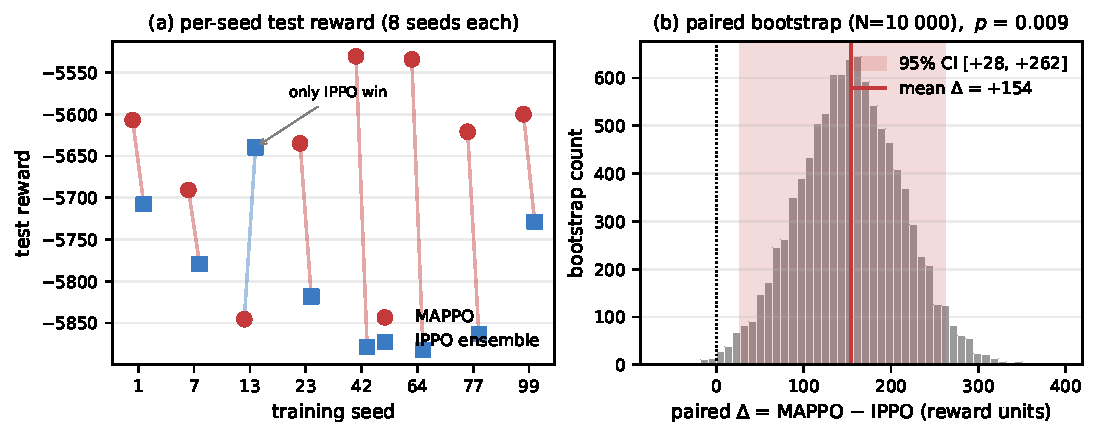
\includegraphics[width=\columnwidth]{figure1.pdf}
\caption{(a) Per-seed test reward for MAPPO (circles) and the IPPO
ensemble (squares) across eight seeds; paired lines connect
seed-matched runs. Seed 13 is the only seed where IPPO wins.
(b) Paired-bootstrap distribution ($10\,000$ resamples) of the mean
$\Delta = \mathrm{MAPPO}-\mathrm{IPPO}$ delta; the 95\,\% CI
$[+28,+262]$ excludes zero ($p=0.009$).}
\label{fig:bootstrap}
\end{figure}

\noindent\textbf{Statistical significance.} A paired bootstrap
(10\,000 resamples of seed-matched MAPPO\,$-$\,IPPO deltas) places
the architectural gap at \textbf{$+154$ reward units, 95\,\% CI
$[+28,+262]$, one-sided $p\!=\!0.009$}. Seven of eight seeds favour
MAPPO (Fig.~\ref{fig:bootstrap}); the only counter-example
(seed~13) is the seed where MAPPO converged to a slightly more
aggressive USR-usage policy (0.67\,\% unsafe, 364 flips vs the
average 0.52\,\%, 290 flips).

\noindent\textbf{Per-cluster transfer.} MAPPO's win concentrates on
the lowest-load cluster (c0, mean load 0.108~Gbps, $+6.6$\,\%) and
on mid-load clusters where the IPPO ensemble's per-cluster PPO
failed to leave always-DPDK because per-cluster data alone was
insufficient signal (c5 $+8.6$\,\%, c7 $+4.3$\,\%, c4 $+3.4$\,\%).
MAPPO's shared actor---trained simultaneously on the data-rich
clusters c0/c1/c4/c6/c7---generalises the
``USR-at-low-predicted-load'' rule to c5, where IPPO never escapes
DPDK. MAPPO wins on 7 of 10 clusters, ties on 1, and loses by
$\leq\!9$\,\% on the remaining 2.

\noindent\textbf{Classical-baseline sensitivity.} Sweeping the
hysteresis band over $\{5, 10, 20, 50, 100\}$~Mbps identifies
band\,=\,50 as the strongest classical operating point
($-6262$); band $\leq\!10$ over-switches
(unsafe~$>\!1.1$\,\%); band\,=\,100 collapses to always-DPDK
because $t_{\mathrm{down}}\!\to\!0$. \emph{No setting of the band
closes the gap to MAPPO.} A complementary cooldown sweep on MAPPO
around the default $(\mathrm{period}\!=\!4, \mathrm{cost}\!=\!0.5)$
confirms the result is not load-bearing on the cooldown
hyperparameters (full sweep tables in the supplementary
material).

% ---------------------------------------------------------------------------
\section{Conclusion}
\label{sec:conclusion}
% ---------------------------------------------------------------------------
Per-site DPDK/USR realisation switching across heterogeneous edge
clusters is a cooperative-MARL problem whose architectural choice
matters more than the algorithm. Under a physics-grounded reward
that unifies steady-state and switching energy, MAPPO with a
shared-parameter actor and centralised critic statistically beats
both an independent-PPO ensemble ($p\!=\!0.009$) and the swept-best
classical hysteresis controller (629 reward units) on a 10.5-day
held-out test slice from a calibrated digital twin. The advantage
concentrates on data-poor mid-load clusters, consistent with
cross-cluster policy transfer through the shared actor. Trained
checkpoints, the digital twin, and an interactive dashboard are
released for reproducibility.\footnote{Public artefact URL to be
inserted at submission.}

% ---------------------------------------------------------------------------
% References (manual `thebibliography` until BibTeX entries are
% finalised; verify entries before final submission).
% ---------------------------------------------------------------------------
\begin{thebibliography}{99}

\bibitem{ref:comcom}
[TO~VERIFY] Source paper for the paper-aligned reward shape
(SEC + asymmetric switching cost + QoS penalty),
COMCOM-S-26-00430.

\bibitem{ref:mappo}
C.~Yu, A.~Velu, E.~Vinitsky, J.~Gao, Y.~Wang, A.~Bayen, and Y.~Wu,
``The surprising effectiveness of PPO in cooperative multi-agent
games,'' in \emph{Adv.\ Neural Inf.\ Process.\ Syst.\ (NeurIPS)},
2022.

\bibitem{ref:ppo}
J.~Schulman, F.~Wolski, P.~Dhariwal, A.~Radford, and O.~Klimov,
``Proximal policy optimization algorithms,'' \emph{arXiv preprint
arXiv:1707.06347}, 2017.

\bibitem{ref:gae}
J.~Schulman, P.~Moritz, S.~Levine, M.~Jordan, and P.~Abbeel,
``High-dimensional continuous control using generalized advantage
estimation,'' in \emph{Int.\ Conf.\ Learn.\ Represent.\ (ICLR)},
2016.

\bibitem{ref:forecaster}
[TO~VERIFY] Upstream traffic forecaster (\texttt{UpfTrafficForecaster})
producing per-cluster predictions used in this work.

\bibitem{ref:upfndt}
[TO~VERIFY] Upstream digital-twin and threshold-derivation framework
(\texttt{UPF\_NDT}); also the source of the RAPL-measured DPDK/USR
activation durations.

\bibitem{ref:sb3}
A.~Raffin, A.~Hill, A.~Gleave, A.~Kanervisto, M.~Ernestus, and
N.~Dormann, ``Stable-Baselines3: Reliable reinforcement learning
implementations,'' \emph{J.\ Mach.\ Learn.\ Res.}, vol.~22,
no.~268, pp.~1--8, 2021.

\end{thebibliography}

\end{document}
